\section{Physics Modeling}

The dataset collected by the ATLAS experiment is both limited and opaque.
It is limited because of the enormous effort required to run the LHC and operate the experiment.
It is opaque because so many aspects of the collision are inaccessible to observation, from the initial state of the protons to the intermediate physics processes.
Even the collision's final state is imperfectly known due to the limited acceptance and detection efficiency of the experiment.
In light of these challenges, it is helpful to simulate collisions computationally and the resulting detector response to produce simulated datasets.

Simulated datasets are used for several purposes.
Because events are simulated based on particular Feynman diagrams, it is possible to explore how those diagrams contribute to the dataset.
% Use 1) composition
This is particularly helpful when considering kinematic distributions, such as the dilepton invariant-mass spectra.
In these, the simulation illuminates the composition of both signal and background distributions.
% Use 2) signal model
With this information, many choices may be made to improve the performance of the analysis.
These include choices of the criteria that define the fiducial region of a search, or choices of the functional form that well describes the shapes of the background distributions.
In the \hmm analysis, simulated datasets are used to develop a multivariate discriminant tuned to identify signal-like events.
% Use 3) signal model
The simulated signal dataset is also useful to model the shape and amplitude of the signal when performing hypothesis tests.
This provides a map from a signal hypothesis's theoretical descriptions to experimentally testable predictions about event yields and distributions.
% Use 4) Systematics
Finally, simulated events provide a means to understand the performance and systematic uncertainties of the ATLAS detector itself.

Since they share many aspects, this section describes how simulated datasets are produced for both the \hmm and \nr analyses.
The procedure begins with event simulation, where a particular set of interactions are represented based on their matrix element.
This step is performed by an \emph{event generator} program.
The matrix element only describes the immediate interaction, or hard-scatter process, and the associated underlying event.
The event generation produces a particle description of the immediate aftermath of a collision. This is described in Section \ref{sec:evtGen}.
After this, the strongly charged particles undergo parton showering and hadronization.
The next step in the simulation describes these processes and results in a set of long-lived particles. This is described in Section \ref{sec:hadronization}.
The final step is the propagation of these particles through the magnetic field and detectors of the experiment.
This is performed with a simulation of the detector's materials described in Section \ref{sec:geant}.

\subsection{Event Generation} \label{sec:evtGen}

An event generator is a program that randomly samples several probability density functions (PDFs) in order to describe a set of possible collision events.
In its present usage, they are concerned with producing events corresponding to the hard-scattering process of a particular Feynman diagrams, but not the long-term evolution of the final state particles.
The PDFs sampled include the parton distribution functions that describe the initial state of interactions.
They also include the normalized matrix elements under consideration, which describes the likelihood for particular final states to occur.
Through repeated sampling, the Monte-Carlo method, the set events begin to represent the events one might expect from a particular set of initial state conditions.

Different event generators are available with various strengths and weaknesses.
The work of this thesis uses samples produced primarily by \sherpa \cite{Gleisberg:2008ta} and \powheg \cite{Alioli:2010xd,Frixione:2007vw}.
In two instances, \pythia \cite{pythia8} and \madgraph \cite{Alwall:2014hca} are selected to produce signal events.

The parton distribution function also varies depending on the process being simulated.
Most simulated datasets are produced with NNPDF3.0NLO \cite{Ball:2014uwa}, and CT10 \cite{ct10}.
In some cases, variations such as NNPDF23LO \cite{Ball:2012cx} or NNLOPS \cite{Hamilton:2013fea} are used.
When unavoidable, PDF4LHC \cite{Butterworth:2015oua} is used.

% % hmm 
% Sherpa 2.2.1 with NNPDF3.0 DY
% Sherpa 2.2.2 with NNPDF3.0 diboson
% Powheg-Box v2 using NNPDF3.0 and Pythia 8.186 for parton showing and A14 param set ttbar
% Powheg-box v2 using NNLOPS (NNLO), PDF4LHC15, Pythia8 showerHadron ggH
% Powheg-box v2, Pythia8 shower/had NLO VBF and VH
% Powhegbox LO ggZH
% MG5_aMC@NLO with NNPDF3.0NLO and Pythia8 showerHadron

% % NR
% Powheg-Box and CT10, NLO: DY
% Powheg-Box and NNPDF3.0 NLO: top
% Sherpa 2.2.1 with CT10: Diboson
% Powheg-Box and NNPDF23LO, NLO: LO DY for Signal


\subsection{Showering and Hadronization} \label{sec:hadronization}

The hard-scattering process describes a final state, including strongly charged and unstable particles.
These can radiate photons, quarks, and gluons in a process called parton showering (PS).
In principle, the initial state partons may also radiate and contribute to PS in an event.
The PS calculation focuses on soft radiation, while the matrix element is used to describe hard radiation.
This division is necessary since the matrix element tends toward infinity as the radiation becomes increasingly soft.
A mixing scheme is used to blend these to produce an accurate description of PS.

Eventually, the final-state quarks and gluons separate and hadronize into color-neutral states.
Since this process is difficult to model from physical principles, it is based on a statistical sampling of the phase space available to the final state particles.
Programs make use of PDFs that have been adjusted to match experimental observation.

There are several programs capable of modeling PS and hadronization.
The event generator \pythia is also capable of modeling both and is used to process most simulated datasets.
The program \evtgen \cite{Lange:2001uf} complements \pythia by modeling bottom and charm hadron decays.
The event generator \sherpa is also used in some cases for PS.
The result of these steps is events of relatively stable ($c\tau>1$~cm) particles, including photons, leptons, and hadrons.
Before reconstruction, such an event is referred to as the \emph{truth} event and consists of \emph{truth particles}.
Truth events are useful in order to evaluate the performance of the detector, as well as the accuracy of the following analysis.


% % Hmm
% For MC using Pythia8-> EvtGen 1.2.0 used for bottom/charm decays

\subsection{Detector Simulation} \label{sec:geant}

\begin{figure}[h!]
\captionsetup[subfigure]{position=b}
\centering
\subfloat[][]{{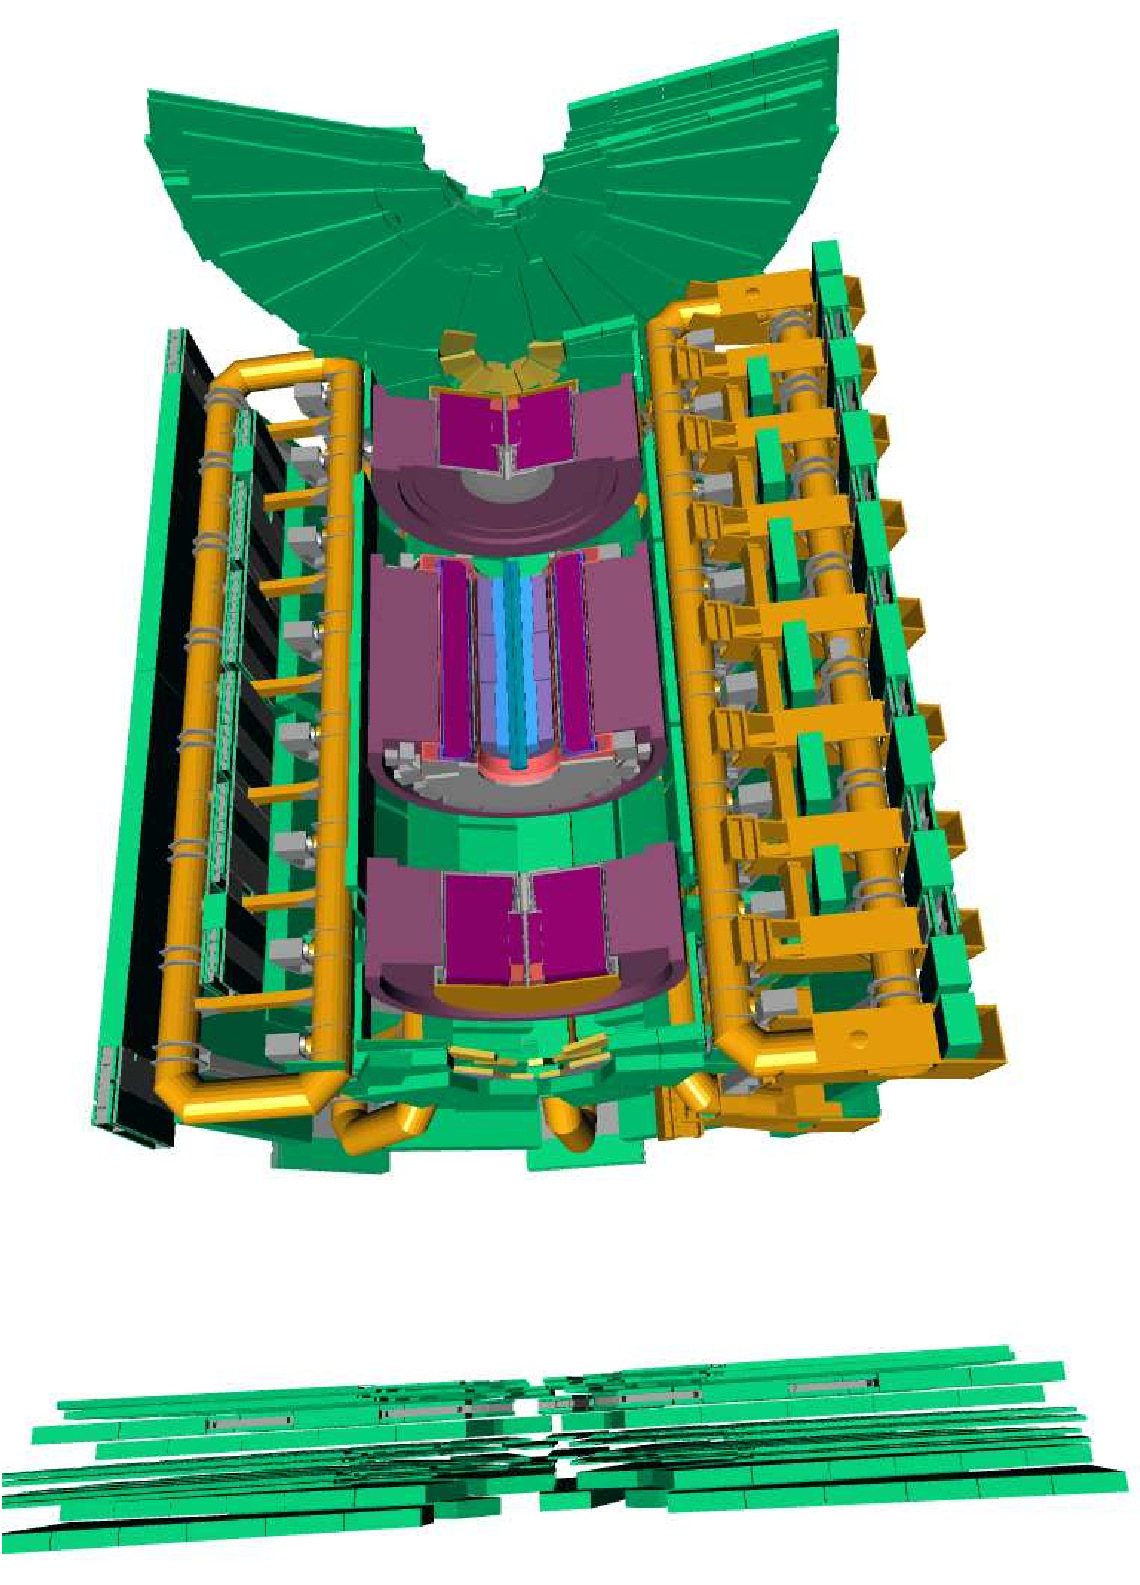
\includegraphics[angle=-90,width=0.7\textwidth]{figures/pheno/atlasSim.pdf}}}
\caption{Graphical representation of the \geant simulation of the ATLAS detector.}
\label{fig:atlasGeantSim}
\end{figure}

The final step is to simulate the response of ATLAS to the simulated events.
This is the closest approximation to the measured dataset.
It is also the most computationally intensive step, as it necessitates a full simulation over time of particle interactions within ATLAS.
The simulation is based on \geant \cite{geant}, and is part of the ATLAS simulation infrastructure \cite{SOFT-2010-01}.
The \geant model of ATLAS consists of nearly five million simulated volumes of both detectors and supporting structures in which particles may interact.
An illustration of the components of the simulation is shown in Figure \ref{fig:atlasGeantSim}.
A three-dimensional map of the magnetic field within ATLAS is included in the simulation as well.
The simulation transports truth particles through the magnetic field and detector volumes.
When a particle enters a detector volume, its interactions with the detector and the corresponding readout electronics are simulated.
The output of the readout electronics simulation is of the same format as the physical detector's output.
After this point, the simulation can be routed through reconstruction identically to data.

